\chapter{Situation Aware Person Following}
\label{chapter:following_situation_aware}

Most simply put, \textit{Situation Awareness (SA)} is knowing what is going on around you. Endsley \cite{endsley2000situation} defines three steps for SA: perception, comprehension and projection. Perception is detecting the situation by perceiving cues, comprehension is combining and interpreting information and projection is forecasting future events. In this section, we discuss SA for person following behavior for mobile robots. In the Chapter \ref{chapter:person_following}, we presented the basic following behavior, where the robot follows the person strictly from behind, while maintaining a fixed distance. The related works on person following discussed in Section \ref{sec:following_related_work} uses the same principle: the robot uses the person to calculate a target position and blindly follows the human irrespective of the situation. Although this method is sufficient for some scenarios, it can easily lead to socially awkward situations. For example, consider for a person following robot that its users stops just outside a door. In this case, the robot would occupy the doorway, blocking other people's passage, however thinks it is doing its task well because it maintains a fixed distance to the user. If the robot knows what the person intends to do, it can anticipate those actions and suitably adjust its behavior.

Person following can be used in different contexts, such as for carrying luggage in airports or groceries in a supermarket. We showed in Chapter \ref{chapter:map_annotation} that semantic maps that include landmarks and waypoints could be used to communicate goals between the robot and the user.  The stored semantic information can also be used to facilitate robot navigation. We specifically focus on three scenarios:

\begin{enumerate}
\item Joining a group of people
\item Labeling landmarks during the Tour Scenario
\item Passing Doors
\end{enumerate}

The robot behaviors for each of these scenarios are modeled and executed via triggered events, inspired by Cakmak \cite{cakmak2011using}. Handling of an event during following is implemented as a sequence of four phases:

\begin{enumerate}
\item Signal: Robot detects an event using perceptual cues
\item Approach: Robot moves to a position better suited to the task
\item Execution: Robot and Human execute for the task
\item Release: Robot detects the end of event
\end{enumerate}

When the event ends, robot continues with Basic Following behavior described in Section \ref{sec:following_basic_person_following}. With this methodology, robot uses the three steps of SA: Perception for detecting the start and ending of an event, Comprehension for interpreting where it should move to and what the task is, and Projection to estimate the future goals of the person. In this chapter, we study three scenarios that could be encountered while the robot is following the person. In Section \ref{sec:following_joining_group}, we first show how the robot moves when the followed person stops and talks with someone else. In Section \ref{sec:following_landmark_labeling}, we study the following behavior for labeling landmarks during the Tour Scenario. In Section \ref{sec:following_door_passing}, we look at how the robot should handle door passages.


\section{Joining a Group}
\label{sec:following_joining_group}

While the robot is following a person, one of the scenarios that could be encountered is when the followed person interacts with some other person. If the basic following method is used, the robot would stay behind the person and that could lead to an awkward formation where the robot is left out of the group (see Figure \ref{fig:group_problem} for an example). Our proposed solution to this problem is for the robot to join the group of people using engagement rules. Joining a group with has been addressed previously \cite{althaus2004navigation,setti2015f}, however none was in the person following context.

\begin{figure}[ht!]
\centering
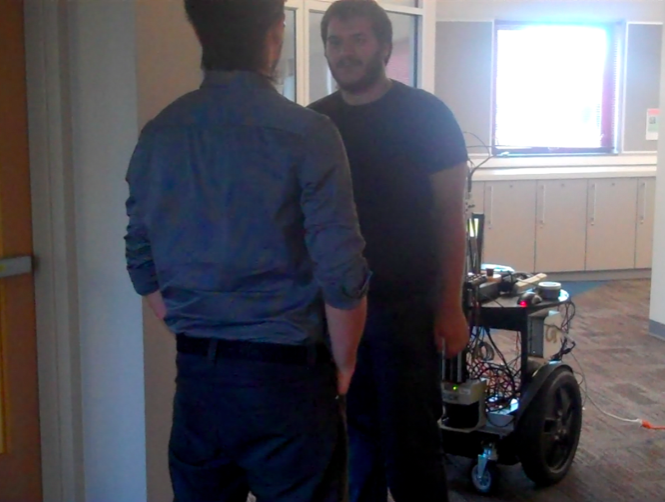
\includegraphics[width=0.5\textwidth]{pics/group_problem}
\caption{The problem that occurs when the followed person stops and interacts with another person is illustrated. The robot is left out of the group when it does not detect or react to this social situation.}
\label{fig:group_problem}
\end{figure}


Our solution to this problem is to choose a position for the robot to stay during the conversation. Our choice of the position is guided by Keldon's F-Formations. Keldon studied how people assemble and what formations they assume while they are interacting. In Keldon's representation the space is divided in three regions as can be seen in Figure: \ref{fig:keldon}. \textit{o-space} is the empty space surrounded by people,  \textit{p-space} contains the participants and \textit{r-space} is the outer area beyond the \textit{o-space}. Keldon studied commonly encountered formations such as L-formation, circular, face-to-face and side-by-side formations.

\begin{figure}[ht!]
\centering
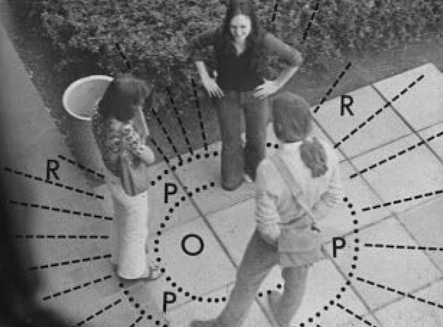
\includegraphics[width=0.5\textwidth]{pics/keldon}
\caption{Definition of space around people according to Keldon's F-Formation representation of group formations}
\label{fig:keldon}
\end{figure}

In our approach, when the robot detects the existence of a group formation, it samples poses on the \textit{p-space}, scores them and chooses a collision-free goal pose. When the interaction ends and the group formation is broken, the robot continues the basic following behavior. The execution phases for this behavior as well as the behavior transitions are given in Table \ref{table:situation_aware_list_group}.



\begin{table}[ht!]

    \caption{Conditions to trigger phases when the user is involved with the Joining a Group Event during following.}

    \centering
    	
  \begin{tabular}{l |  m{10cm}}    
    \toprule    
    Signal & {$dist(user, groupcenter)<threshold$}\\       
	                           & {$speed(user)\sim 0$} \\
	                           & {person roughly facing group}\\ \midrule		                           		                                
    Approach & {Optimal Goal: in the \textit{p-space} in the circular formation}\\       \midrule
    Execution & {The group interacts with each other, including the robot}\\  \midrule
    Release & {$dist(user, groupcenter)>threshold$}\\ 
    \bottomrule
  \end{tabular}
    \label{table:situation_aware_list_group}
\end{table}

We follow the Signal/Approach/Task/Release procedure for the design of this behavior. The Signaling phase is triggered whenever the user is close to another person or a group of people. The user must have close to zero speed to enable signaling for this behavior, because the user may walk past the group. After the robot detects the signal, we sample positions around the group to locate a ``suitable" goal pose for the robot. A pose that is collision free but that gives the robot highest chance of interaction is favored. We use a utility function that scores candidate goal points. Intuitively, a pose that is close to both people and could see both is considered a suitable goal pose. We sample points $360^{\circ}$ around the \textit{p-space}, for a fixed sampling resolution. 

\begin{figure}[ht!]
\centering
%
        \subfigure[]{%           
           \label{fig:situtation_aware_joining_group_0}
           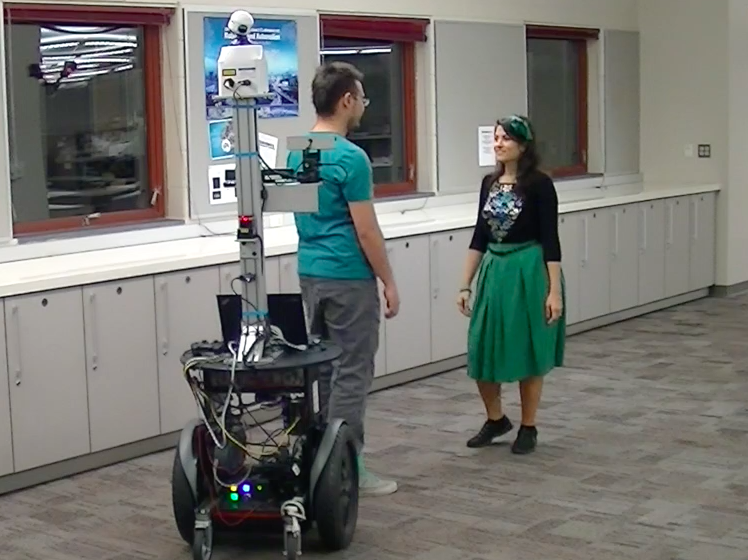
\includegraphics[width=0.475\textwidth]{pics/group_demo_1}
        } 
         \subfigure[]{%           
           \label{fig:situtation_aware_joining_group_1}
           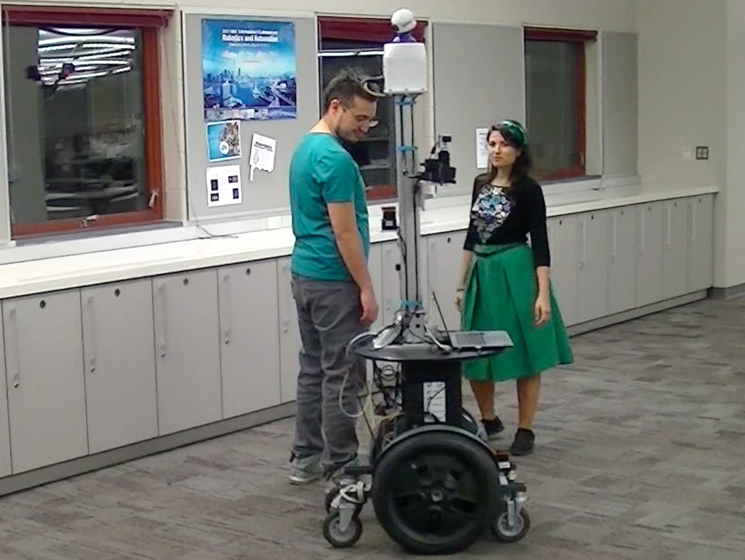
\includegraphics[width=0.48\textwidth]{pics/group_demo_2}
        } \\
        \subfigure[]{%
        	\label{fig:situtation_aware_joining_group_2}
            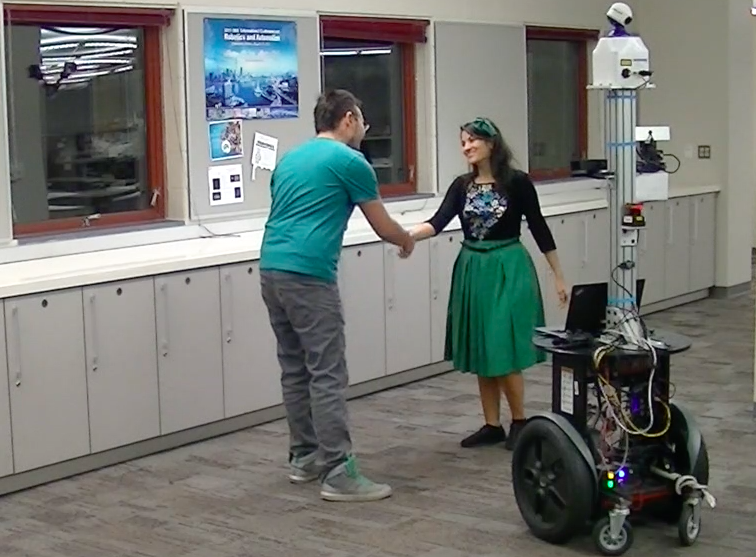
\includegraphics[width=0.48\textwidth]{pics/group_demo_3}
        }%\\        
        \subfigure[]{%           
           \label{fig:situtation_aware_joining_group_3}
           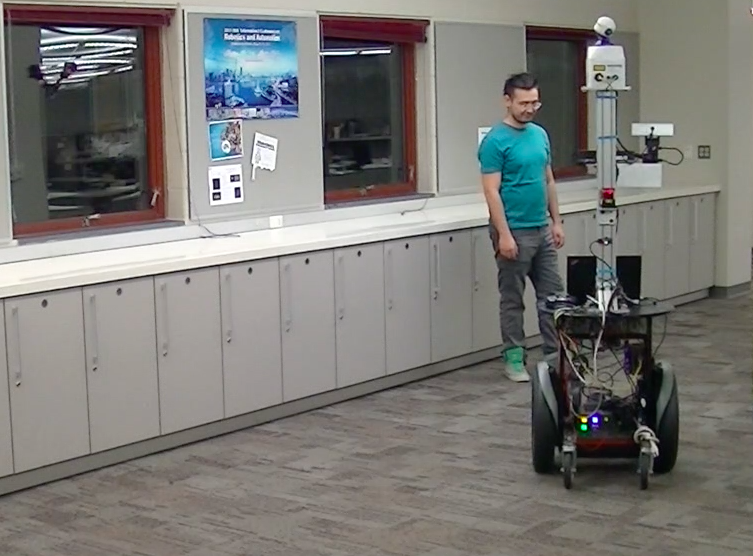
\includegraphics[width=0.49\textwidth]{pics/group_demo_4}
        }
    \caption{Demonstration of the robot joining a group when the followed person interacts with a group of people. The robot is initially following the user throughout the environment and keeping a fixed distance of $1.2m$ to the user. a) Signal phase: The user has stopped and is in the cloxe proximity to to another person. b) Approach phase: The robot calculates and navigates to a goal position, so it can potentially interact with people in the group. c) Execution phase: The interaction happens. c) Release phase: user moves away from the group and basic following behavior continues.}
   \label{fig:situtation_aware_joining_group}
\end{figure}

Every sampled position $p$ has a score of:
\[
Score(p) = 1.0 - Cost_{visibility}(p) - Cost_{obstacle}(p)
\]
Where we define the costs as:
\begin{align} 
\begin{split}
Cost_{visibility}(p)&=dist(user,person)/(dist(p,person)-dist(p,user)) \\
Cost_{obstacle}(p)&=max(local\_cost(p),global\_cost(p))
\end{split}
\end{align}

The local and global costs are fetched from the ROS costmaps, normalized to [0.0-1.0] interval. The sample with the highest nonnegative score is chosen as the goal position. The orientation of the robot is chosen as looking toward the center of all the people in the group. After the goal pose is determined, the robot is commanded to navigate there. During the Execution phase, interaction that potentially involves the robot occurs. Whenever the user leaves the group, then the Release phase is executed. The robot continues tracking the user with the basic following method.

The steps of this behavior implemented on a real robot is shown in Figure \ref{fig:situtation_aware_joining_group}.

\section{Following For Labeling}
\label{sec:following_landmark_labeling}

One of the problems during the Tour Scenario is that as the robot is following the user, it does not have any information about the task. This leads to awkward situations when the user wants to label a landmark or object, because the robot can not perceive the pointing gesture or the object/landmark of interest at the same time when it is following from behind all the time. This situation is illustrated in Figure \ref{fig:landmark_labeling_example}.

\begin{figure}[ht!]
\centering
        \subfigure[]{%           
           \label{fig:label_ex_1}
           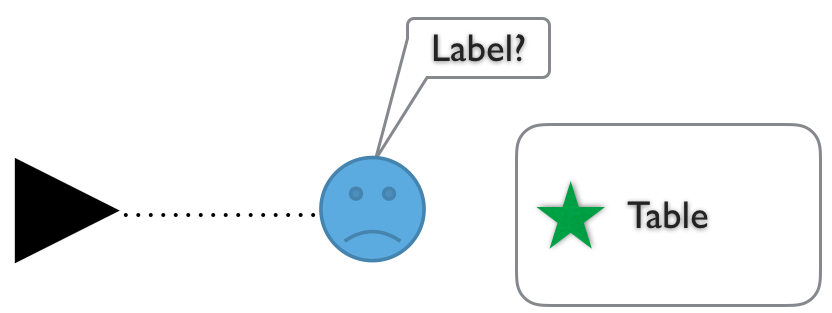
\includegraphics[width=0.58\textwidth]{pics/label_ex_1}
        } \\
        \hspace*{3cm}
         \subfigure[]{%           
           \label{fig:label_ex_2}
           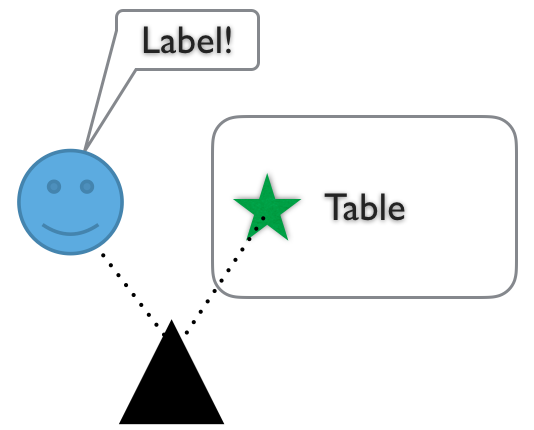
\includegraphics[width=0.38\textwidth]{pics/label_ex_2}
        } 
    \caption{Caption}
   \label{fig:landmark_labeling_example}
\end{figure}

 The robot behavior can be more intelligent in those cases if the robot can predict ahead of time when the user is going to label landmark. The robot follows the phase transitions defined in Table \ref{table:situation_aware_list_landmark} for this scenario.
 
\begin{table}[ht!]

	\caption{Conditions to trigger phases when the user is involved with the Landmark Labeling Event during following.}
	
		\centering
		
  \begin{tabular}{l |  m{10cm}}
    \toprule    
    Signal & {$dist(user, convex hull(landmark))<threshold$}\\       
	                           & {$speed(user)\sim 0$} \\
	                           & {person roughly facing landmark}\\ \midrule		                           		                                
    Approach & {Optimal Goal: Close to both the landmark and person, facing in between}\\       \midrule
    Execution & {User points and labels landmark}\\  \midrule
    Release & {$dist(user, convex hull(landmark))>threshold$}\\ 
    \bottomrule
  \end{tabular}
    \label{table:situation_aware_list_landmark}
\end{table}


\begin{figure}[ht!]
\centering
%
        \subfigure[]{%           
           \label{fig:situtation_aware_landmark_labeling0}
           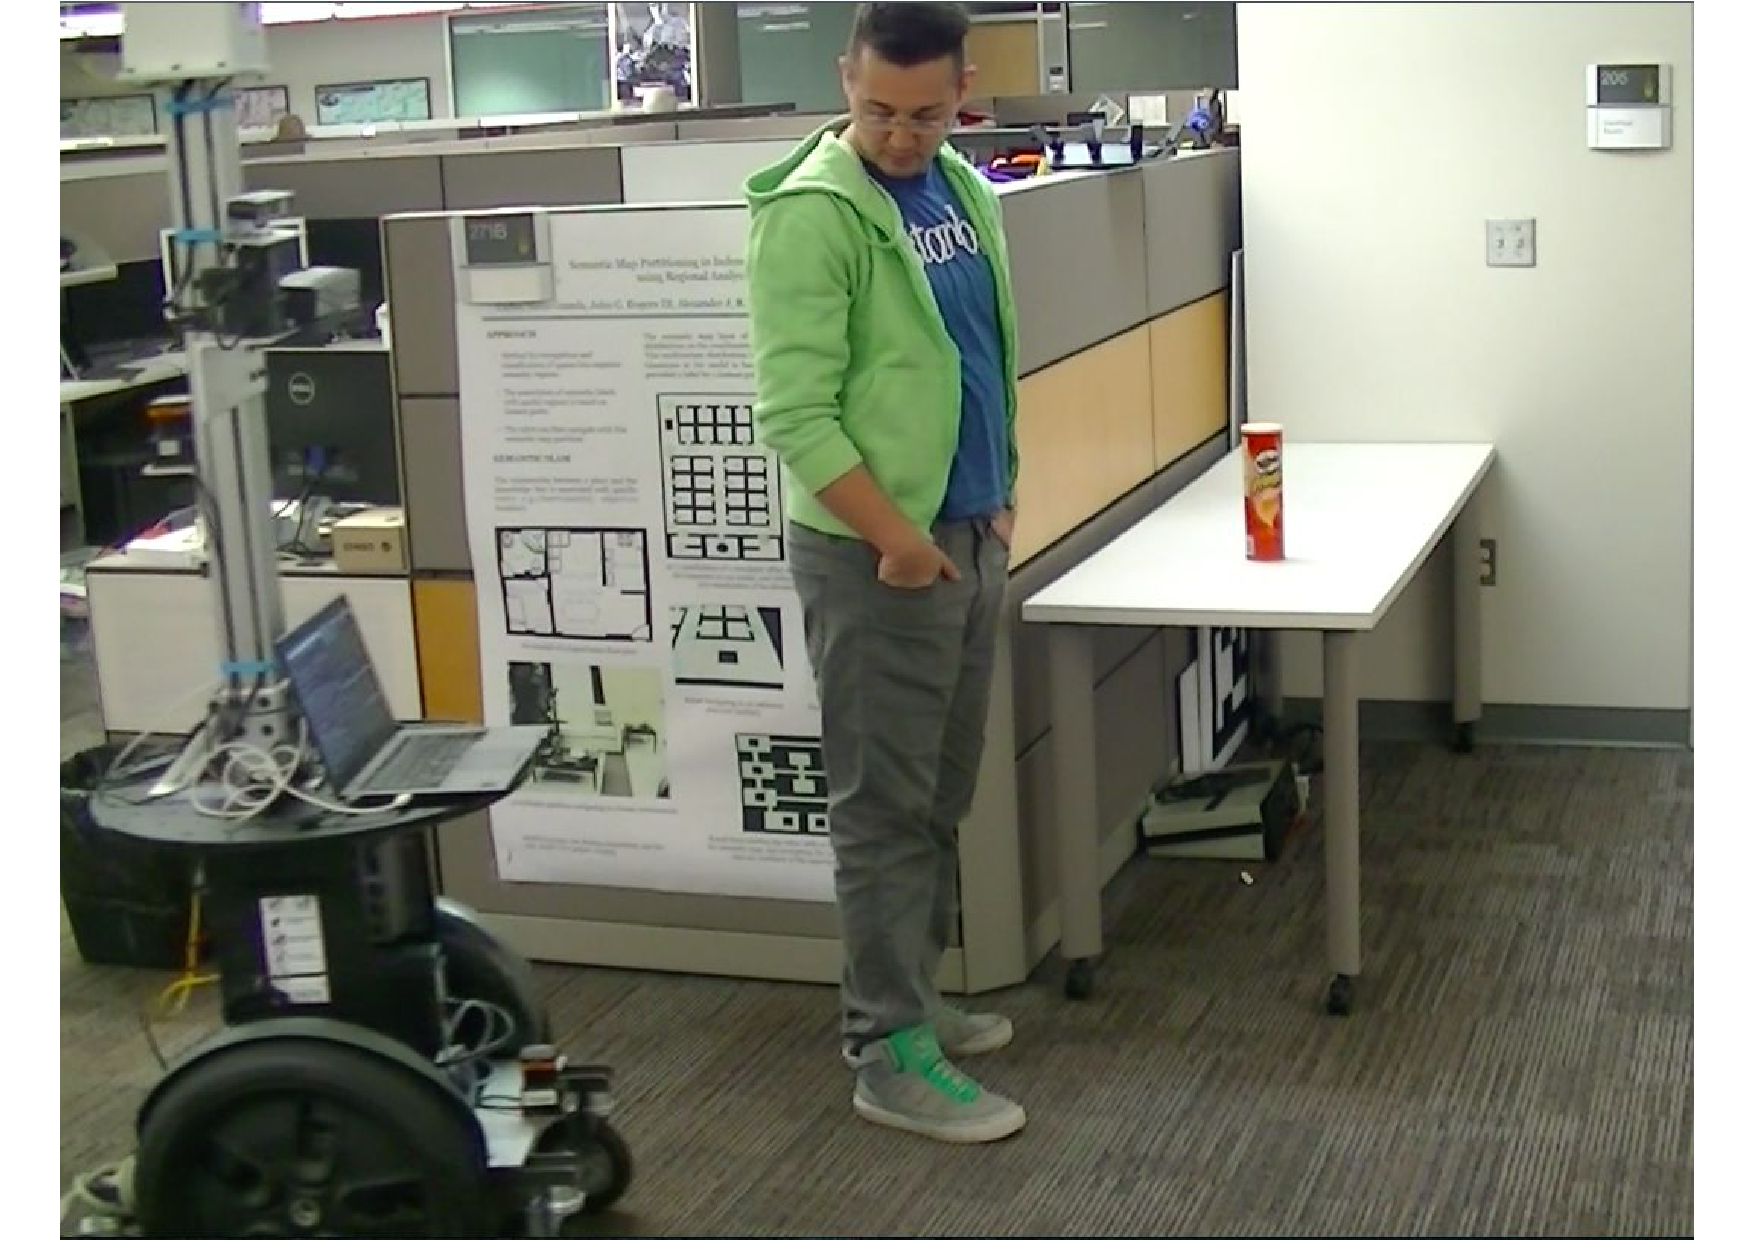
\includegraphics[width=0.475\textwidth]{pics/sit_table_00}
        } 
         \subfigure[]{%           
           \label{fig:situtation_aware_landmark_labeling2}
           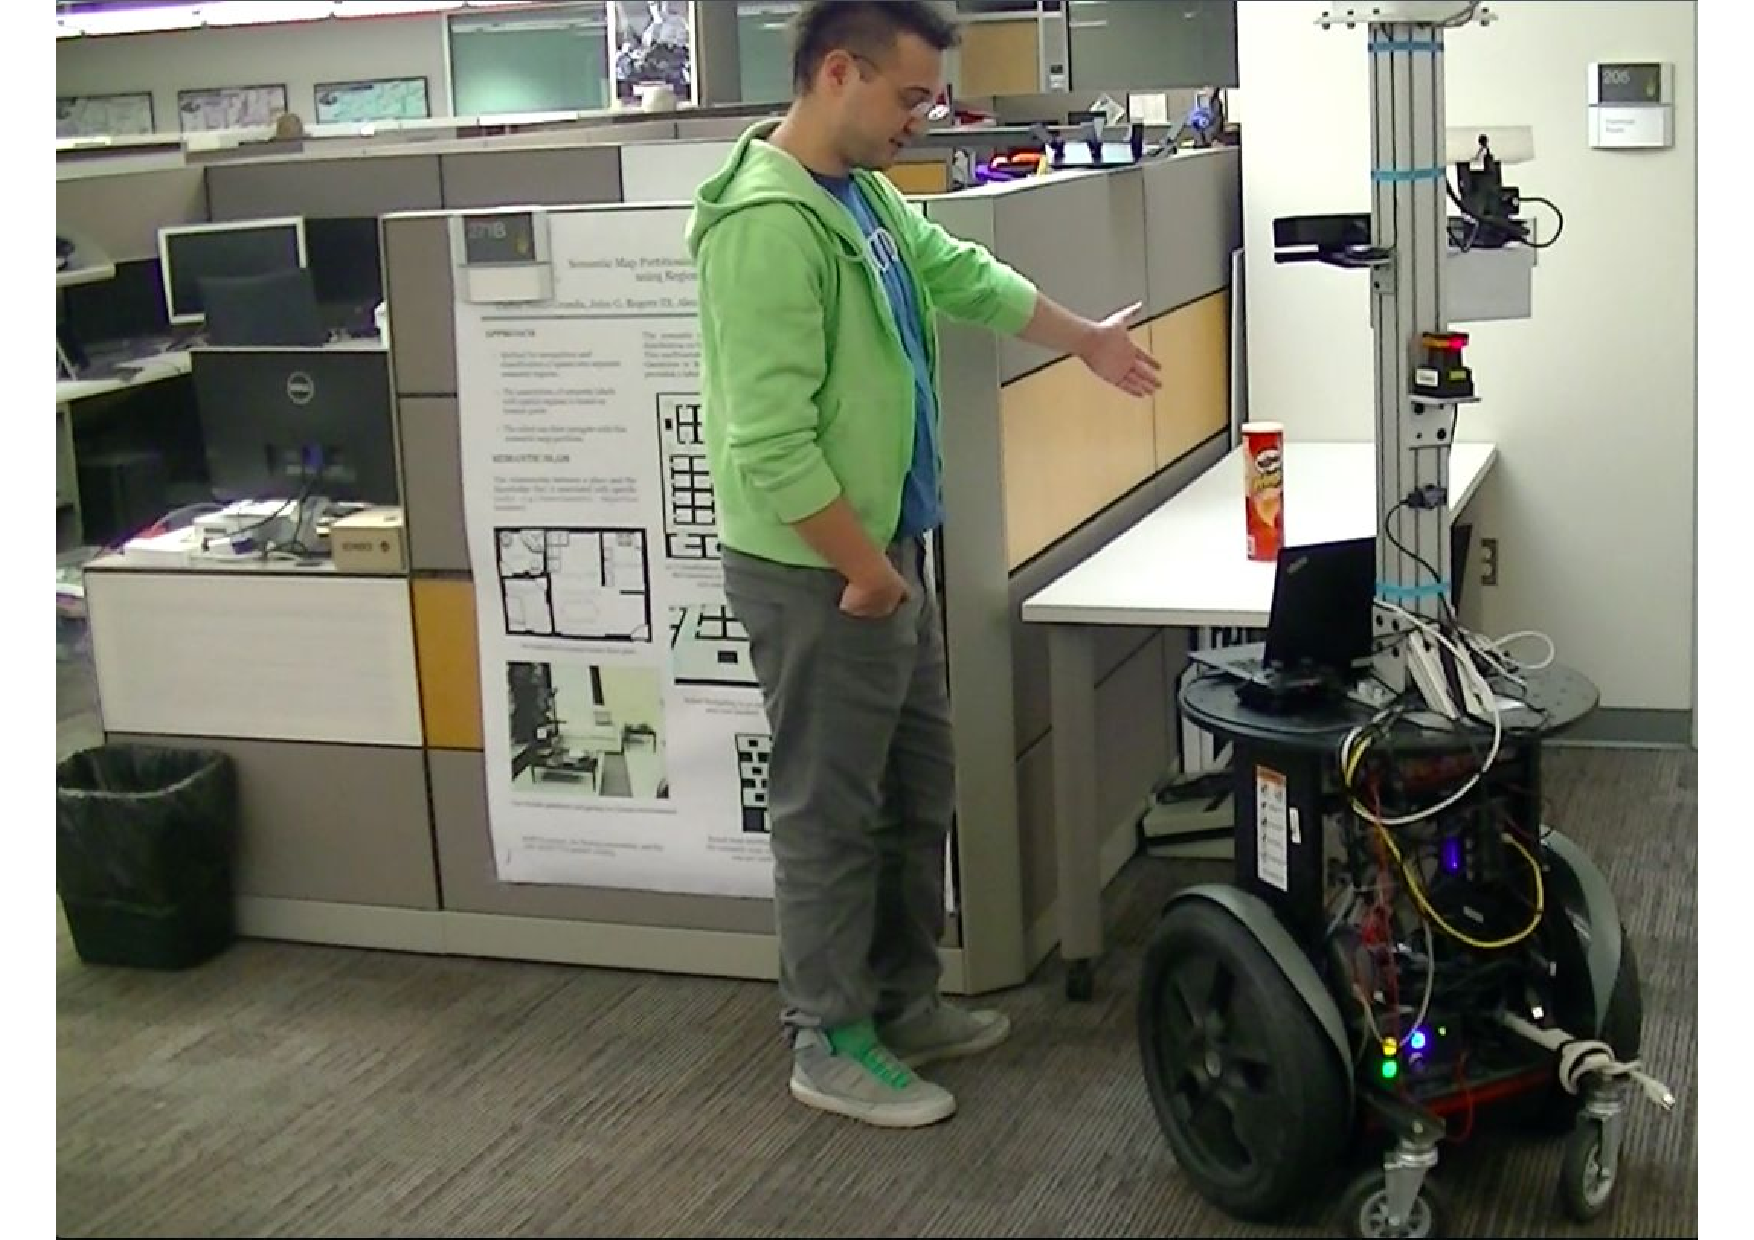
\includegraphics[width=0.48\textwidth]{pics/sit_table_02}
        } \\
        \subfigure[]{%
        	\label{fig:situtation_aware_landmark_labeling3}
            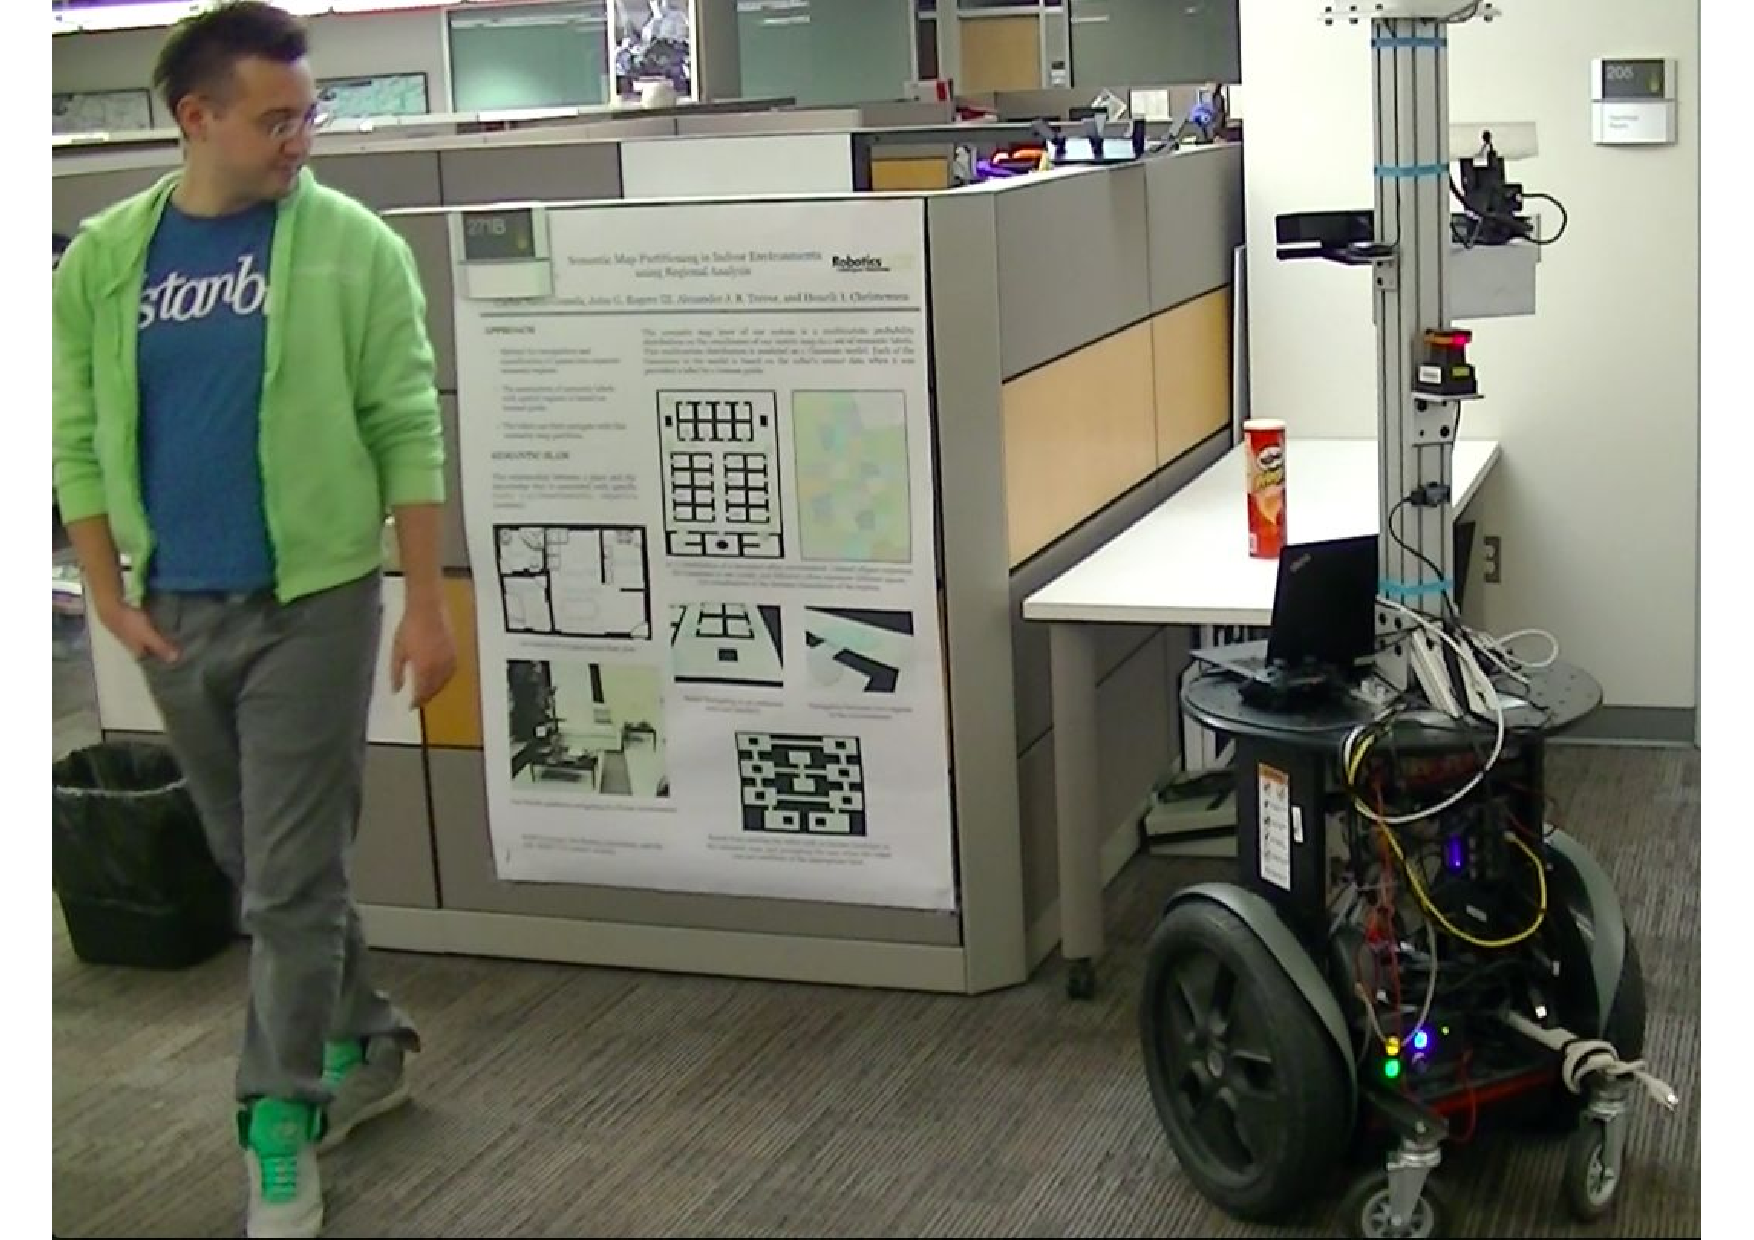
\includegraphics[width=0.48\textwidth]{pics/sit_table_03}
        }%\\        
        \subfigure[]{%           
           \label{fig:situtation_aware_landmark_labeling4}
           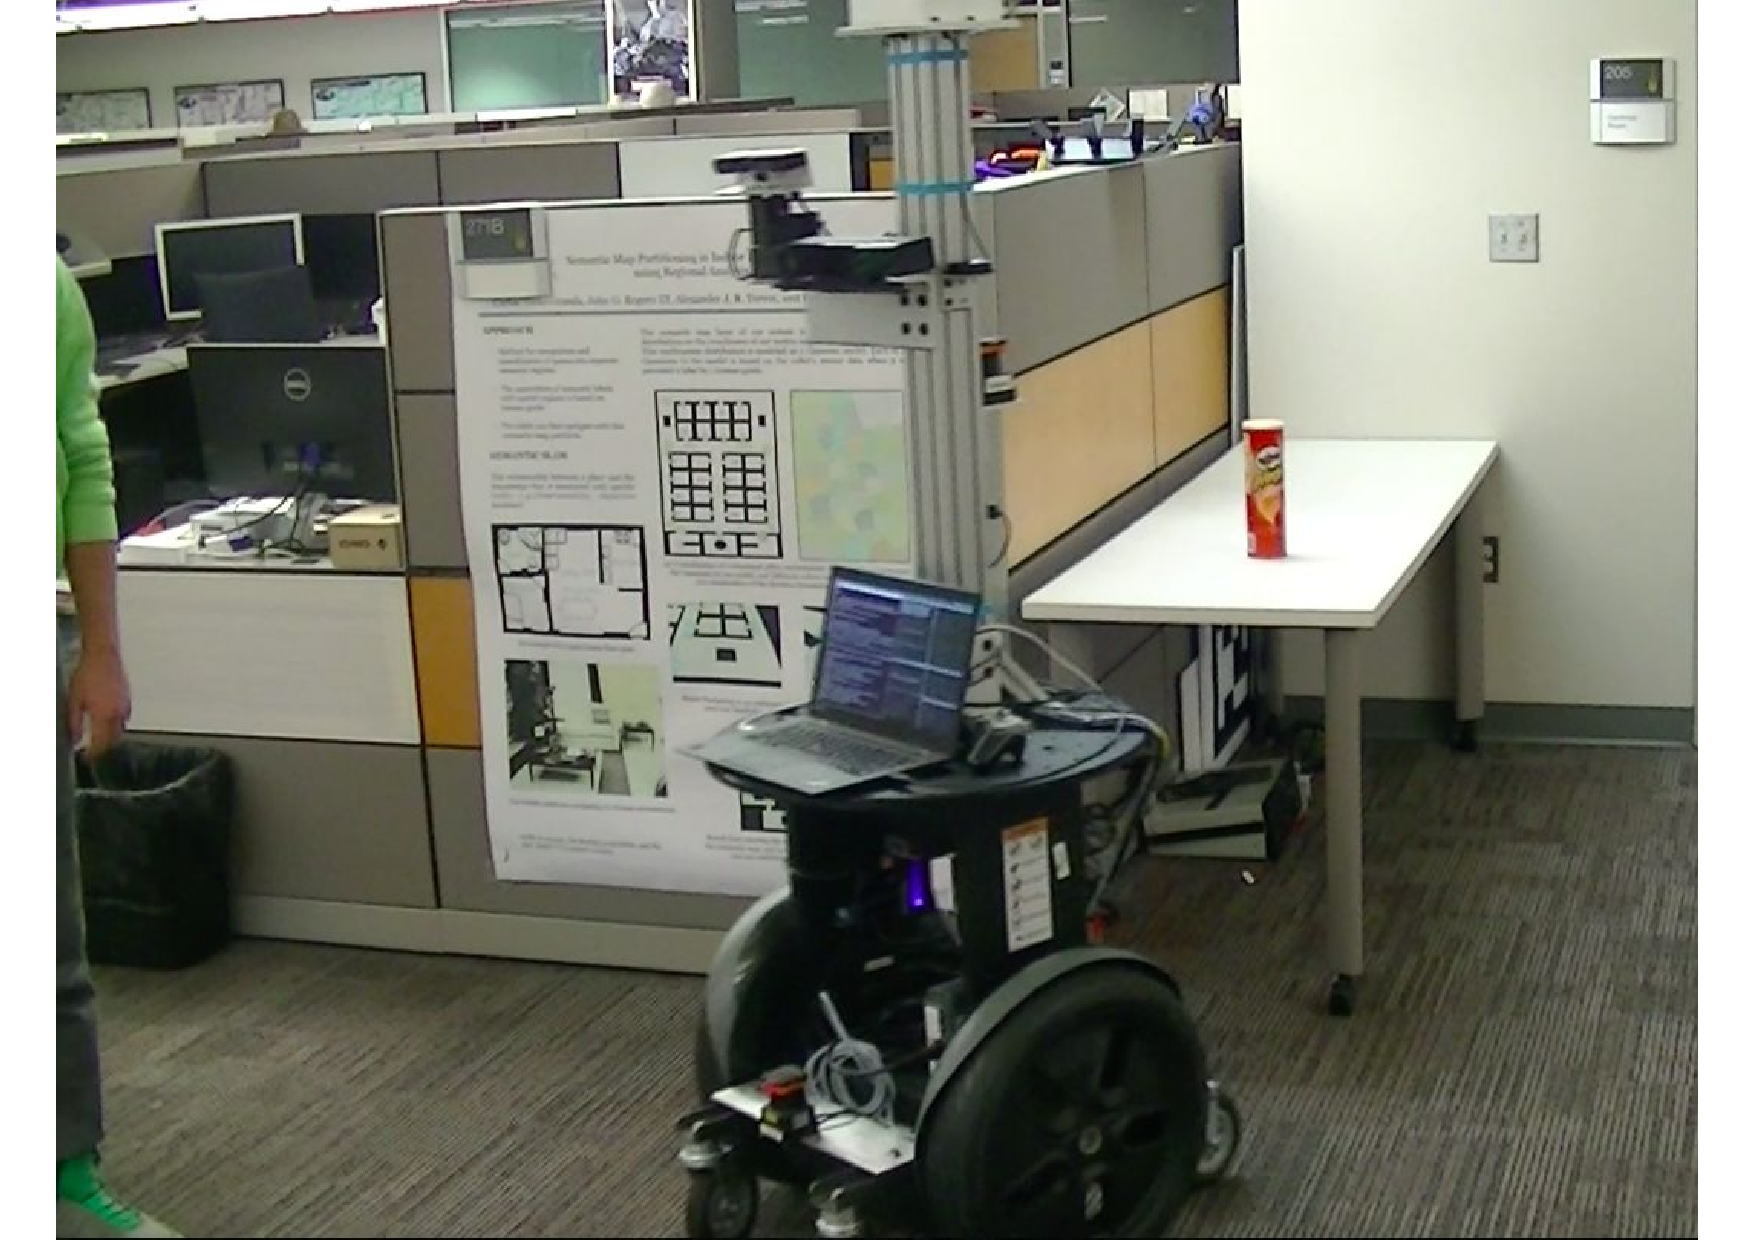
\includegraphics[width=0.49\textwidth]{pics/sit_table_04}
        }
    \caption{Demonstration of situation awareness for the Tour scenario. The robot is following the user throughout the environment and keeping a fixed distance of $1.2m$ to the user. a) Signal phase: The user has stopped and is in the cloxe proximity to the convex hull of the table. b) Approach phase: The robot calculates and navigates to a goal position, so it can perceive the pointing gesture and target. Execution phase: The user points out to the object on the table. c) Release phase: user moves away from the table d) Basic following behavior continues.}
   \label{fig:situtation_aware_landmark_labeling}
\end{figure}

Our approach relies on detecting whenever labeling is going to happen, and position the robot base so it has a better chance to perceive both the pointing gesture and the object/landmark of interest. Our methodology for this scenario is similar to the joining a group behavior as presented in Section \ref{sec:following_joining_group}. Instead of sampling points around the group of people, for the landmark labeling behavior we sample points around a circle that includes the user and the centroid of the convex hull of the landmark.

To go over the phases, this behavior is triggered when the user has stopped nearby an unlabeled landmark or object and facing it. A goal position that is close to both the landmark and person, facing in between is found and the robot navigates there. Then the user can execute the labeling task via pointing gestures. After the task is completed, the robot waits until the user to leaves the vicinity of the landmark. When that happens, the robot continues the Tour scenario by continuing to follow the user. If, during any of the phases, the person tracking fails, it informs the user so following can be restarted. The phases and conditions for this behavior are summarized in Table \ref{table:situation_aware_list_landmark}. The situation awareness for labeling landmarks is implemented on the Segway robot for the Tour Scenario. Snapshots from a demonstration for this is shown in Figure \ref{fig:situtation_aware_landmark_labeling}.

\section{Door Passing}
\label{sec:following_door_passing}

When the user approaches a door during following, the situation can easily become problematic if the robot continues with the basic person following behavior. For example, if the user intends to close an open door or open a closed door, the robot might end up blocking the movement of the door. Moreover, a deadlock situation occurs when the user wants to go through a door with spring-loaded hinges. In that case, the user would need to hold to door to keep it open, and because the distance between the robot and the user is less than the following threshold, the robot would stay still and won't pass the door. A robot SA should be aware of this possibility and take appropriate action. 

\begin{table}[ht!]
	\caption{Conditions to trigger phases when the user is passing through a door during following.}
	\centering
  \begin{tabular}{l |  m{10cm}}    
    \toprule    
    Signal & {$dist(user, convexhull(door))<threshold$}\\         
    	      & {$speed(user)\sim 0$} \\
	      & {User performs pointing gesture towards the passage}\\ \midrule	                           
    Approach & {Optimal Goal: A position on the other side of the door that doesn't block the doorway}\\       \midrule
    Execution & {Robot and user meet at the same side of the door}\\  \midrule
    Release & {$dist(user, convexhull(door))>threshold$ }\\ 
    \bottomrule
  \end{tabular}
    \label{table:situation_aware_list_door}
\end{table}


Opening, closing or passing through a door, and detecting these actions require a sophisticated recognition and system. However the robot can assume that any of those actions are possible when the user is approacing the door. In our approach, the robot can continiously monitor the user's proximity to the doors using the semantic map, if the user labeled door landmarks beforehand. Our approach can handle doors with spring-loaded hinges, even though it does not have a model of the door except the convex hull of its plane.

\begin{figure}[ht!]
\centering
%
        \subfigure[]{%           
           \label{fig:situtation_aware_door_passing0}
           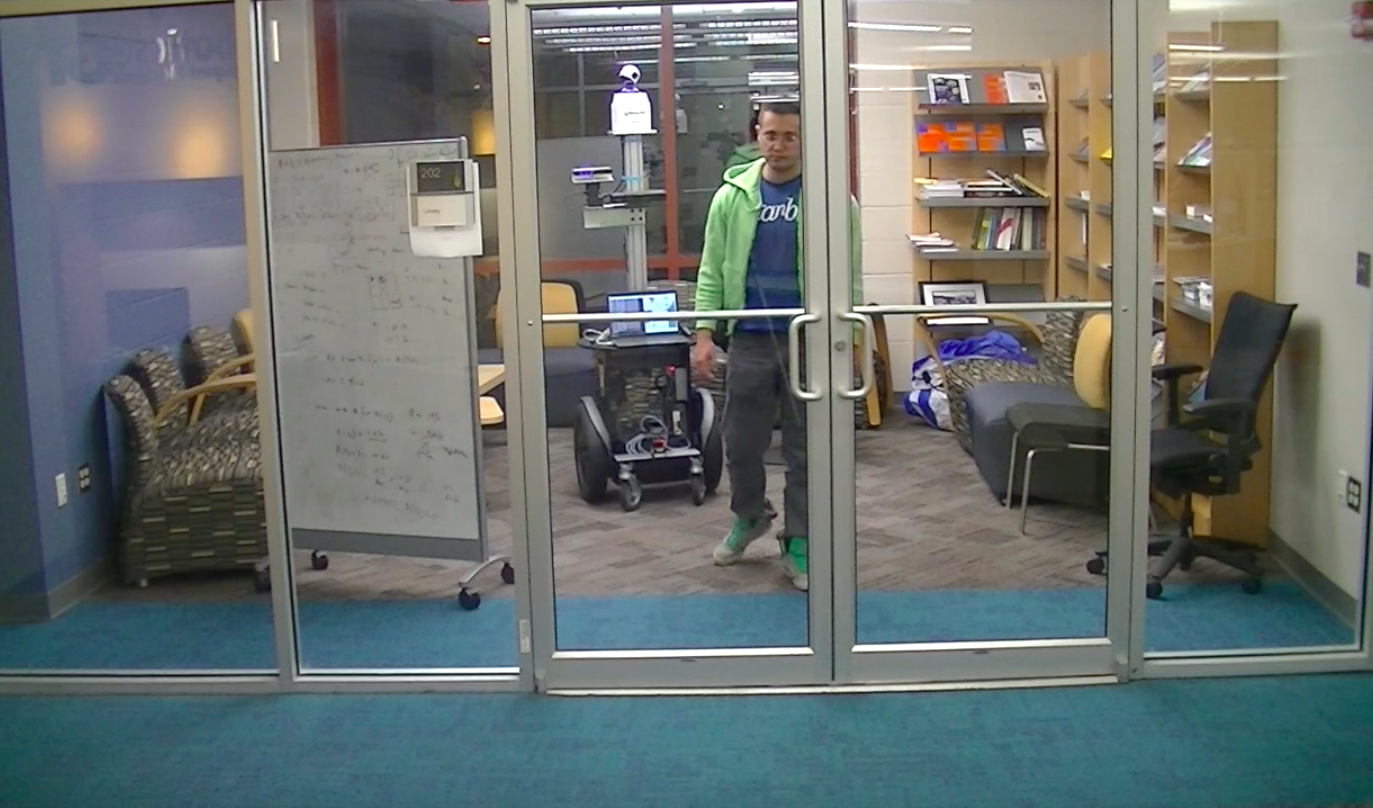
\includegraphics[width=0.475\textwidth]{pics/sit_door_00}
        } 
        \subfigure[]{%           
           \label{fig:situtation_aware_door_passing1}
           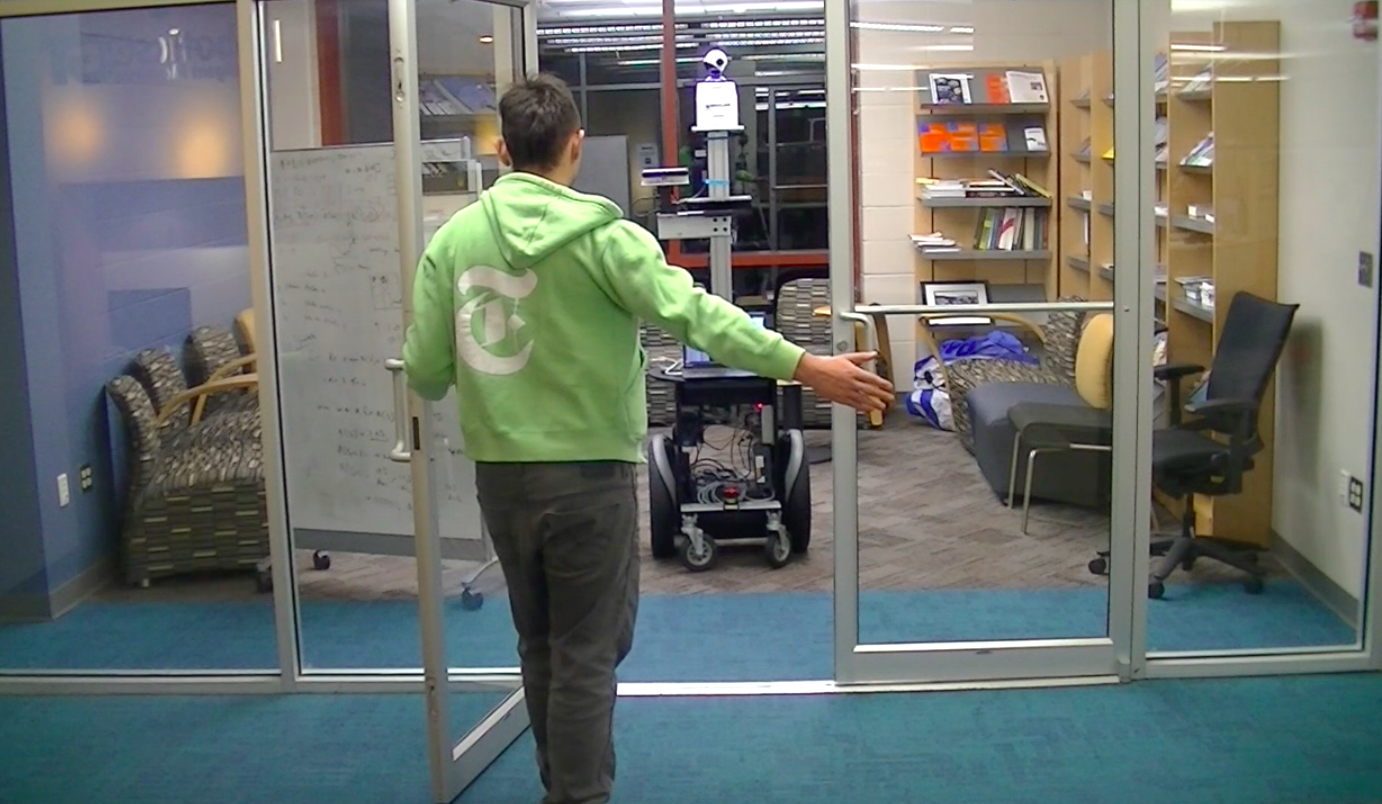
\includegraphics[width=0.48\textwidth]{pics/sit_door_01}
        } \\
        \subfigure[]{%
        	\label{fig:situtation_aware_door_passing2}
            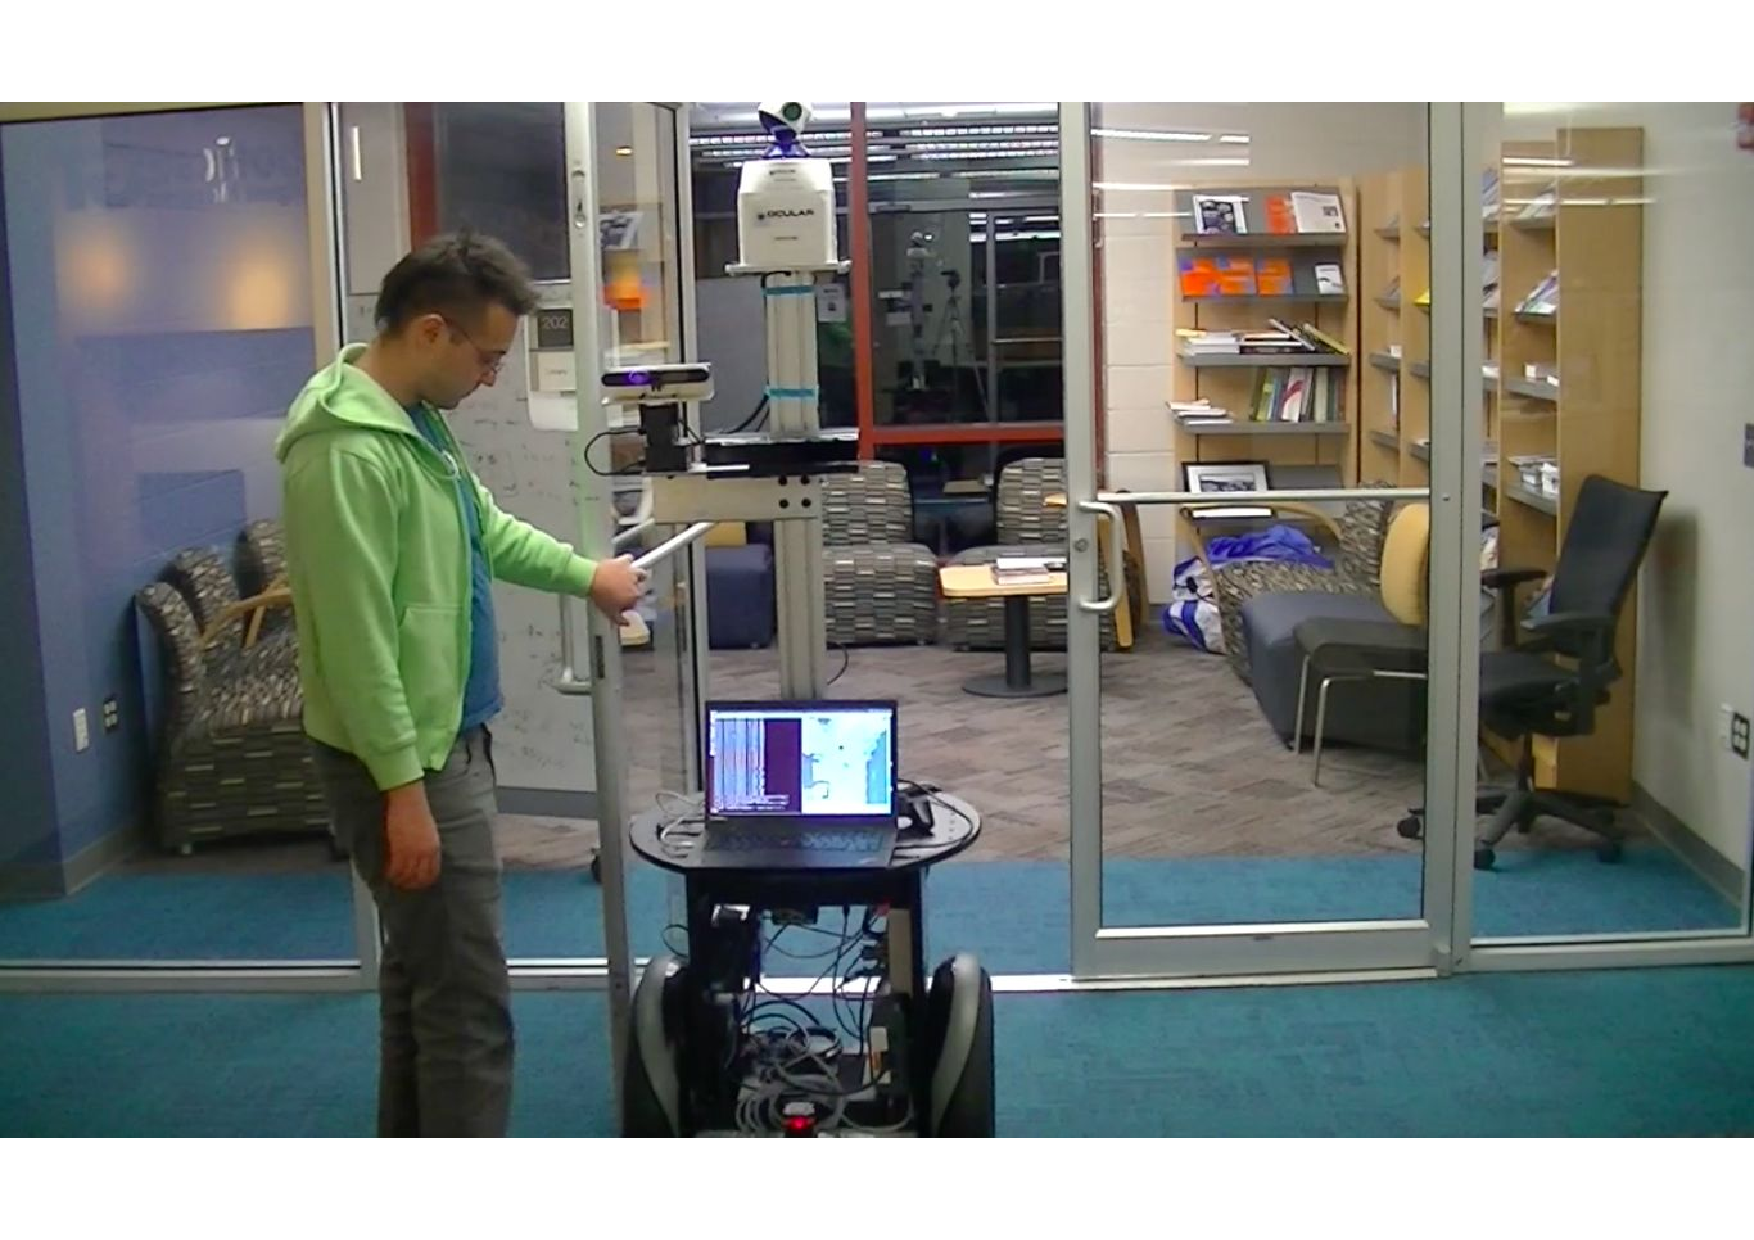
\includegraphics[width=0.48\textwidth]{pics/sit_door_03}
        }%\\        
        \subfigure[]{%           
           \label{fig:situtation_aware_door_passing3}
           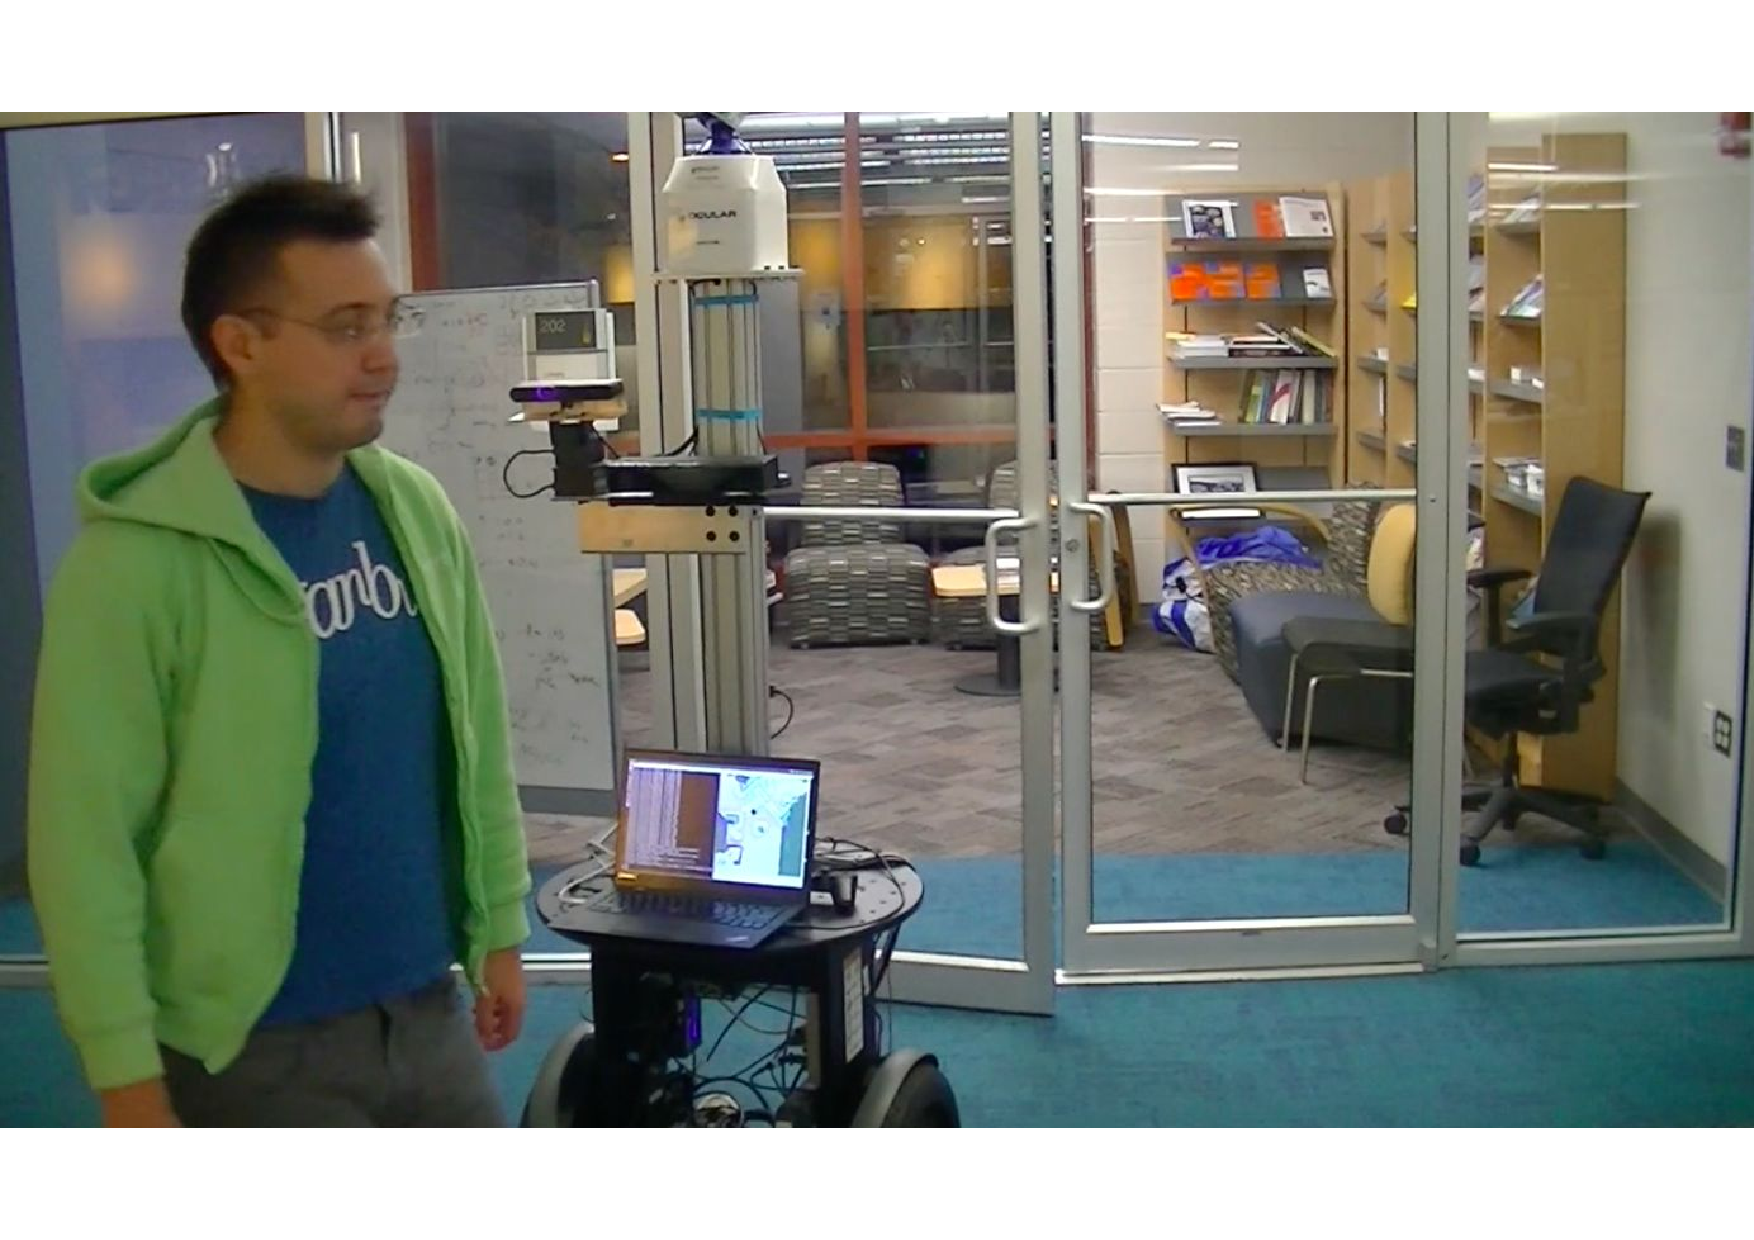
\includegraphics[width=0.49\textwidth]{pics/sit_door_04}
        }
    \caption{Demonstration of situation awareness for door passing during person following. It is assumed that the user previously added the door as a labeled landmark to the semantic map via the Tour Scenario. This is a swing door with spring loaded hinges, so it would close if not kept open actively. a) The robot is following the user by keeping a fixed distance in between. b) Signal phase: The user has stopped, is in close proximity to the door and performed a pointing gesture toward the other room. c) Approach Phase: The robot passes the door while the user is holding the door}
   \label{fig:situtation_aware_door_passing}
\end{figure}

The phases and conditions for door passing situation are summarized in Table \ref{table:situation_aware_list_door}. The robot takes action when the user is nearby a door and performs a pointing gesture towards it, to signal that the robot should pass from the door (Signal Phase). If the action is not signaled, the robot continues with basic following during the door passage. After the detection of a pointing gesture, a goal position is calculated (Approach Phase). The goal positions are sampled on the other side of the door, that is guaranteed not the block the opening/closing of the door. A collision-free position with the least obstacle cost sample is chosen as the goal point. Note that while the robot is moving, it does not necessarily keep a fixed distance to the user anymore. After the robot reaches the goal, it waits for the person to pass the door (Execution Phase). After the user moved away from the door, the basic following behavior takes over. The situation awareness for this scenario is implemented on the Segway robot. The snapshots from the behavior can be seen in Figure \ref{fig:situtation_aware_door_passing}.